%=====================================================================
\section{Lecture 5: Nakajima--Zwanzig, and why the memory kernel is a self-energy}
\label{sec:lec5}

The Nakajima--Zwanzig (NZ) equation is an exact, closed equation of motion for
$\rhoS(t)$. It is derived in five lines with a projection operator, and its memory kernel
$K$ looks at first like a formal object. The content of this lecture is that $K$ is
exactly the sum of the irreducible diagrams of \cref{sec:lec4}, so that the NZ equation is
the Dyson equation of the real-time expansion. We then evaluate $K$ at second order for
the qubit and recover the Bloch--Redfield description, with every rate and shift expressed
through $S$ and $\chi$.

\subsection{The projection and the exact equation}
\label{sec:nz-derivation}

Define the Nakajima--Zwanzig projector~\cite{Nakajima1958,Zwanzig1960}
\begin{equation}
  \Pc X=\rhoB\otimes\Tr_B X,\qquad \Qc=1-\Pc,\qquad \Pc^2=\Pc .
  \label{eq:P}
\end{equation}
$\Pc$ keeps the ``relevant'' part, the reduced state tensored with the fixed reference bath
state. Three facts follow from $[H_B,\rhoB]=0$ and $\avg{B}=0$:
\begin{equation}
  \Pc\Lc_S=\Lc_S\Pc,\qquad \Pc\Lc_B=\Lc_B\Pc=0\ \text{on the range of }\Pc,\qquad \Pc\Lc_I\Pc=0 .
  \label{eq:P-facts}
\end{equation}
(The last one: $\Pc\Lc_I\Pc X=\rhoB\otimes\Tr_B[-i(S B\otimes\rhoB X'-\dots)]\propto\avg{B}=0$.)
Split the von Neumann equation $\dot\rho=\Lc\rho$ into its $\Pc$ and $\Qc$ components:
\begin{equation}
  \partial_t\Pc\rho=\Pc\Lc\Pc\rho+\Pc\Lc\Qc\rho,\qquad
  \partial_t\Qc\rho=\Qc\Lc\Pc\rho+\Qc\Lc\Qc\rho .
\end{equation}
The second is a linear inhomogeneous equation for $\Qc\rho$ with the known source $\Qc\Lc\Pc\rho(s)$:
\begin{equation}
  \Qc\rho(t)=\ee^{\Qc\Lc t}\Qc\rho(0)+\int_0^t\!\dd s\,\ee^{\Qc\Lc(t-s)}\,\Qc\Lc\Pc\rho(s).
\end{equation}
Insert into the first and use \cref{eq:P-facts}:
\begin{equation}
  \boxed{\;\dot\rhoS(t)=\Lc_S\rhoS(t)+\int_0^t\!\dd s\,K(t-s)\,\rhoS(s)+I(t),\qquad
  K(\tau)X=\Tr_B\!\Big[\Lc_I\,\ee^{\Qc\Lc\tau}\,\Qc\Lc_I\big(X\otimes\rhoB\big)\Big],\;}
  \label{eq:NZ}
\end{equation}
with the inhomogeneity $I(t)=\Tr_B[\Lc_I\ee^{\Qc\Lc t}\Qc\rho(0)]$, which vanishes for a
factorized initial state ($\Qc\rho(0)=0$). This is the NZ
equation~\cite[Sec.~9.1]{BreuerPetruccione}. It is exact. Nothing has been assumed about
the strength of the coupling, the Gaussianity of the bath or the size of the system. The
kernel $K(\tau)$ is a superoperator on the system; it depends on $\tau$ only (stationary
bath, time-independent $H$) and it contains the full $\Lc$ inside the exponential, which
is where all the difficulty hides.

\paragraph{Laplace form.}
With $\hat f(z)=\int_0^\infty\dd t\,\ee^{-zt}f(t)$ (Re$\,z>0$), the convolution becomes a product
and \cref{eq:NZ} for the map reads
\begin{equation}
  \boxed{\;\hat\Pi(z)=\frac{1}{z-\Lc_S-\hat K(z)}
  \quad\Longleftrightarrow\quad
  \hat\Pi=\hat\Pi_0+\hat\Pi_0\,\hat K\,\hat\Pi,\qquad \hat\Pi_0=(z-\Lc_S)^{-1}.\;}
  \label{eq:Dyson}
\end{equation}
This is a Dyson equation with $\hat K$ in the role of the self-energy. The next
subsection shows that the analogy is an identity.

\subsection{The kernel is the sum of irreducible diagrams}
\label{sec:nz-irreducible}

\begin{theorem}\label{thm:irreducible}
For the projector \eqref{eq:P}, the NZ kernel is the sum of all diagrams of
\cref{sec:lec4} that cannot be cut between two consecutive vertices without cutting a
line, with the outermost vertices at $0$ and $\tau$:
\begin{equation}
  K(\tau)=\sum_{n\ge1}\;\int_{\tau>t_1>\dots>t_{2n-2}>0}\ \sum_{\text{irreducible pairings of }\{\tau,t_1,\dots,t_{2n-2},0\}}
  \big(\text{vertices}\times\text{lines}\big).
\end{equation}
\end{theorem}

\begin{proof}
Expand $\ee^{\Qc\Lc\tau}$ in powers of $\Lc_I$. Since $\Qc$ commutes with $\Lc_0=\Lc_S+\Lc_B$
(because $\Pc$ does), $\ee^{\Qc\Lc_0s}\Qc=\Qc\ee^{\Lc_0s}$, and the $m$-th order term is
\begin{equation}
  \int_{\tau>s_1>\dots>s_m>0}\Qc\,\ee^{\Lc_0(\tau-s_1)}\,\Qc\Lc_I\,\ee^{\Lc_0(s_1-s_2)}\,\Qc\Lc_I\cdots\Qc\Lc_I\,\ee^{\Lc_0s_m}\,\Qc .
\end{equation}
Sandwiched between the outer $\Tr_B[\Lc_I\cdots]$ and $\Lc_I(X\otimes\rhoB)$, this is the
free (interaction-picture) Wick string of $m+2$ vertices with a factor $\Qc=1-\Pc$ inserted
in every gap between consecutive vertices. Now expand the product of the $(1-\Pc)$'s. A
term with $\Pc$ inserted in a given set $\mathcal C$ of gaps equals, by the definition of
$\Pc$, the Wick string in which the bath is traced and reset to $\rhoB$ at each gap in
$\mathcal C$; by Wick's theorem that is exactly the sum of the pairings in which \emph{no
line crosses any gap in $\mathcal C$}. Hence
\begin{equation}
  \sum_{\mathcal C}(-1)^{|\mathcal C|}\ \#\{\text{pairings with no line across any gap in }\mathcal C\}
  =\#\{\text{pairings with a line across \emph{every} gap}\}
\end{equation}
by inclusion--exclusion, and the right-hand side is the set of irreducible pairings.
\end{proof}

Irreducibility is defined with respect to the reference state $\rhoB$ in $\Pc$: a cut is a
moment at which the bath is \emph{exactly} back in $\rhoB$. A different projector (a
correlated reference state, or Mori's operator projector of \cref{sec:lec8}) gives a
different kernel. The theorem is the real-time version of the statement that the
self-energy is one-particle irreducible; in the superoperator language it goes back to
Schoeller and Sch\"on~\cite{SchoellerSchon1994,Schoeller2000} for fermionic reservoirs and
is the basis of real-time renormalization group methods~\cite{Schoeller2009,Keil2001}; see
also~\cite{LeijnseWegewijs2008,Timm2008} for the explicit comparison with NZ at fourth
order. Two consequences:
\begin{itemize}[itemsep=1pt]
\item $K(0)=K^{(2)}(0)$ exactly: at $\tau=0$ there is no room for internal vertices.
\item $K$ is of order $g^2$ while $\Pi$ is of order $1$; perturbation theory for $K$ is
  perturbation theory for the exponent, which is why NZ at low order already
  captures long-time exponential decay that no finite-order expansion of $\Pi$ can.
\end{itemize}

\subsection{Second order: Born, Redfield, secular, Bloch}
\label{sec:born}

At order $\Lc_I^2$ we drop $\Qc$ in \cref{eq:NZ} (because $\Pc\Lc_I\Pc=0$) and replace
$\ee^{\Qc\Lc\tau}\to\ee^{\Lc_0\tau}$; the result is $K^{(2)}$ of \cref{eq:K2}, now identified as
the first term of the irreducible series. The approximations one layers on top are:
\begin{enumerate}[itemsep=1pt]
\item \textbf{Born (NZ2).} Keep $K\approx K^{(2)}$ in \cref{eq:NZ}, as a time-nonlocal equation.
\item \textbf{Redfield (time-local, nonsecular).} Replace $\rhoS(s)\to\ee^{-\Lc_S(t-s)}\rhoS(t)$
  under the integral (valid when $\rhoS$ changes little, in the interaction picture, over
  the bath correlation time) and extend the upper limit to $\infty$:
  \begin{equation}
    \dot\rhoS=\big[\Lc_S+\Gc^{(2)}_\infty\big]\rhoS,\qquad
    \Gc^{(2)}_\infty=\int_0^\infty\!\dd\tau\,K^{(2)}(\tau)\,\ee^{-\Lc_S\tau}.
    \label{eq:redfield}
  \end{equation}
  This is Redfield's equation~\cite{Redfield1957,WangsnessBloch1953,Bloch1957}; we will
  see in \cref{sec:lec6} that it is the $t\to\infty$ limit of the second-order TCL generator.
\item \textbf{Secular.} Drop the terms of $\Gc^{(2)}_\infty$ that oscillate at $\pm\omega_0$ or $\pm2\omega_0$ in
  the interaction picture. The result is of GKSL form \eqref{eq:GKSL} and generates a
  completely positive semigroup (Davies' theorem~\cite{Davies1974}; see
  \cite[Sec.~3.3.1]{BreuerPetruccione} for the general construction). Without the secular
  step, Redfield can violate positivity at short times.
\end{enumerate}

\begin{exbox}[Example 5.1: the Bloch equations for the qubit]
Apply \cref{eq:redfield} to the kernel \eqref{eq:K2-bloch}. The rotation $\ee^{-\Lc_S\tau}$ acts
on the \emph{input}: $(x_x,x_y)\mapsto(\cos\,x_x+\sin\,x_y,\,-\sin\,x_x+\cos\,x_y)$. Multiplying out
and keeping the secular terms (the $\tau$-integrals of products such as
$S_\tau\cos\omega_0\tau\cos\omega_0\tau$ contain a non-oscillating half; the $cs$ cross terms and
the $\cos^2$-type oscillating halves drop), one finds the Bloch equations
\begin{equation}
  \dot r_z=-\Gamma_1\big(r_z-r_z^{\rm eq}\big),\qquad
  \dot r_\pm=\big(\pm i\tilde\omega_0-\Gamma_2\big)r_\pm,\qquad r_\pm\equiv r_x\pm ir_y ,
  \label{eq:bloch-eqs}
\end{equation}
with
\begin{align}
  \Gamma_1&=\Gamma_\downarrow+\Gamma_\uparrow=2\sin^2\theta\,S(\omega_0),\qquad
  \Gamma_{\downarrow}=2\sin^2\theta\,J(\omega_0)\big[1+n(\omega_0)\big],\quad
  \Gamma_{\uparrow}=2\sin^2\theta\,J(\omega_0)\,n(\omega_0),
  \label{eq:rates-T1}\\
  r_z^{\rm eq}&=-\frac{\chi''(\omega_0)}{S(\omega_0)}=-\tanh\frac{\beta\omega_0}{2},
  \label{eq:rz-eq}\\
  \Gamma_2&=\tfrac12\Gamma_1+\Gamma_\varphi,\qquad \Gamma_\varphi=2\cos^2\theta\,S(\omega{=}0),
  \label{eq:rates-T2}\\
  \tilde\omega_0&=\omega_0+\delta\omega,\qquad
  \delta\omega=2\sin^2\theta\int_0^\infty\!\dd\tau\,S(\tau)\sin\omega_0\tau
  =\frac{\sin^2\theta}{\pi}\,\mathrm P\!\!\int_{-\infty}^{\infty}\!\dd\omega\,\frac{S(\omega)}{\omega_0-\omega}.
  \label{eq:lamb}
\end{align}
Each line is worth a comment.
\begin{itemize}[itemsep=1pt]
\item \Cref{eq:rates-T1}: the population column of $K^{(2)}$ gives
  $\int_0^\infty K_{zz}\dd\tau=-4\sin^2\theta\int_0^\infty S(\tau)\cos\omega_0\tau\,\dd\tau=-2\sin^2\theta S(\omega_0)$. The
  \emph{sum} of the rates is set by the noise at $\omega_0$. Using the FDT,
  $S(\omega_0)=J(\omega_0)[1+2n(\omega_0)]$, which splits into $\Gamma_\downarrow+\Gamma_\uparrow$ as written. This is
  Fermi's golden rule with the $C(\pm\omega_0)$ of \cref{eq:FDT}.
\item \Cref{eq:rz-eq}: the inhomogeneous term is
  $\int_0^\infty K_{z\Id}\dd\tau=-2\sin^2\theta\int_0^\infty\chi(\tau)\sin\omega_0\tau\,\dd\tau=-2\sin^2\theta\,\chi''(\omega_0)$. The
  \emph{difference} of the rates, $\Gamma_\downarrow-\Gamma_\uparrow=2\sin^2\theta\chi''(\omega_0)$, is set by the
  response. The ratio $\chi''/S=\tanh(\beta\omega_0/2)$ is the FDT, and it makes the steady state
  the Gibbs state of $H_S$: detailed balance is the fluctuation--dissipation theorem seen
  from the system. Out of equilibrium (a driven or nonthermal bath), $S$ and $\chi''$ are
  independent and $r_z^{\rm eq}$ defines an effective temperature.
\item \Cref{eq:rates-T2}: pure dephasing samples the noise at zero frequency and
  comes with $\cos^2\theta$; relaxation contributes half its rate to the coherence decay. For
  $S=\sz/2$ one would have $\Gamma_\varphi=\tfrac12\cos^2\theta S(0)$.
\item \Cref{eq:lamb}: the Lamb shift is the Hilbert transform of the \emph{noise} spectrum.
  At $T=0$, $S(\omega)=J(|\omega|)$ and the integral splits into the rotating-wave term
  $\mathrm P\!\int_0^\infty J(\omega)/(\omega_0-\omega)$ and the counter-rotating (Bloch--Siegert) term
  $\int_0^\infty J(\omega)/(\omega_0+\omega)$. The response $\chi'$ drops out of the shift because it is
  even in $\omega$ (\cref{ex:5-2}).
\end{itemize}
For the Lorentzian bath of \cref{sec:lec2} at $T=0$, with $\Omega=\omega_0=1$, $\gamma=0.5$,
$\theta=\pi/4$, $g=0.3$: $\Gamma_\downarrow=0.360$, $\Gamma_\uparrow=0.0055$ (from the negative-frequency
tail), $\Gamma_\varphi=0.0424$, $\Gamma_2=0.225$, $\delta\omega=g^2\sin^2\theta\,\frac{2\Omega}{4\Omega^2+\gamma^2/4}=0.022$. The
script of \cref{sec:numerics} computes $\Gc^{(2)}_\infty$ numerically and reproduces all of these
to three digits (the nonsecular generator gives a precession frequency $1.0219$ versus
$1.0222$ secular).
\end{exbox}

\begin{figure}[t]
\centering
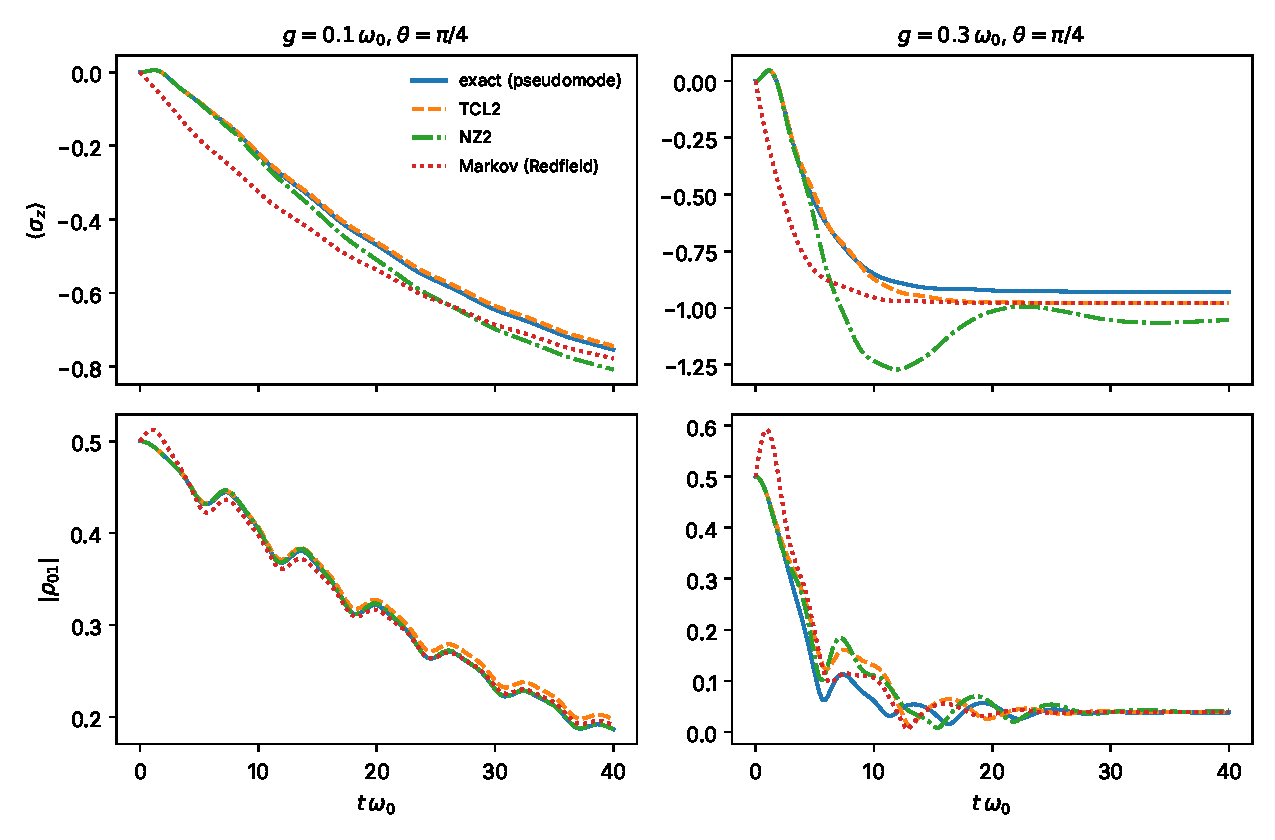
\includegraphics[width=\textwidth]{figures/fig_dynamics.pdf}
\caption{Qubit dynamics in the Lorentzian bath ($\Omega=\omega_0$, $\gamma=0.5\omega_0$, $T=0$,
$\theta=\pi/4$), starting from $\ket{+x}$, for weak (left) and moderate (right) coupling. Exact
(pseudomode) versus the three second-order schemes of this lecture and the next: NZ2
(Born, time-nonlocal), TCL2 (time-local, time-dependent rates) and the Markovian Redfield
limit. At $g=0.3$ the Born kernel drives $\avg{\sz}$ below $-1$, a violation of positivity;
TCL2 stays physical and tracks the exact solution; Markov misses the initial slip and the
coupling-induced shift of the steady state.}
\label{fig:dynamics}
\end{figure}

\Cref{fig:dynamics} compares the three second-order schemes with the exact solution.
Three lessons: (i) at weak coupling all agree, and the Markovian rates of Example~5.1 are
quantitatively right after a transient of duration $\sim1/\gamma$; (ii) the Born kernel used
\emph{nonlocally} (NZ2) is the \emph{worst} of the three at stronger coupling, overshooting
to unphysical states, a well-known pathology~\cite{SmirneVacchini2010}; (iii) the exact
steady state is not the Gibbs state of $H_S$ but the reduced state of the global
equilibrium, which the second-order schemes can only approximate.

\subsection{Beyond second order}

The fourth-order kernel is the sum of the crossed and nested diagrams of
\cref{fig:fourth-order}, each with its full vertex structure (all assignments of
$\cl/\qu$ consistent with the rules, i.e.\ $\qu\qu$ lines carrying $S$ and $\qu\cl$ lines
carrying $-i\chi$). Written out,
\begin{equation}
  K^{(4)}(\tau)=\int_{\tau>t_1>t_2>0}\Big\{V_\tau V_{t_1}V_{t_2}V_0\Big\}_{\text{crossed }(\tau t_2)(t_10)}
  +\Big\{V_\tau V_{t_1}V_{t_2}V_0\Big\}_{\text{nested }(\tau0)(t_1t_2)},
\end{equation}
where $V_{t}$ denotes the vertex at time $t$ (either $-iS^\qu$ or $-iS^\cl$ according to the
line it belongs to),
with free propagators between vertices in the Schr\"odinger picture. For
$\theta=0$ on the coherence it reduces to the crossed and nested integrals of
\cref{eq:dephasing-4th} times $16$. Explicit fourth-order kernels for the spin-boson model
were worked out in the TCL form by Breuer, Kappler and
Petruccione~\cite{BreuerKapplerPetruccione2001}; in the NZ form the bookkeeping is easiest
in Laplace space~\cite{Timm2008}. \Cref{fig:kernels} (left) shows the exact kernel of the
Lorentzian model, extracted numerically from the pseudomode representation as
$\Pc\Lc_I\ee^{\Qc\Lc\tau}\Qc\Lc_I\Pc$, against $K^{(2)}$: the higher orders shift the oscillation
frequency inside the kernel (a self-consistent Lamb shift) and change its damping, but
$K(0)=K^{(2)}(0)$ exactly, as the theorem requires.

\begin{figure}[t]
\centering
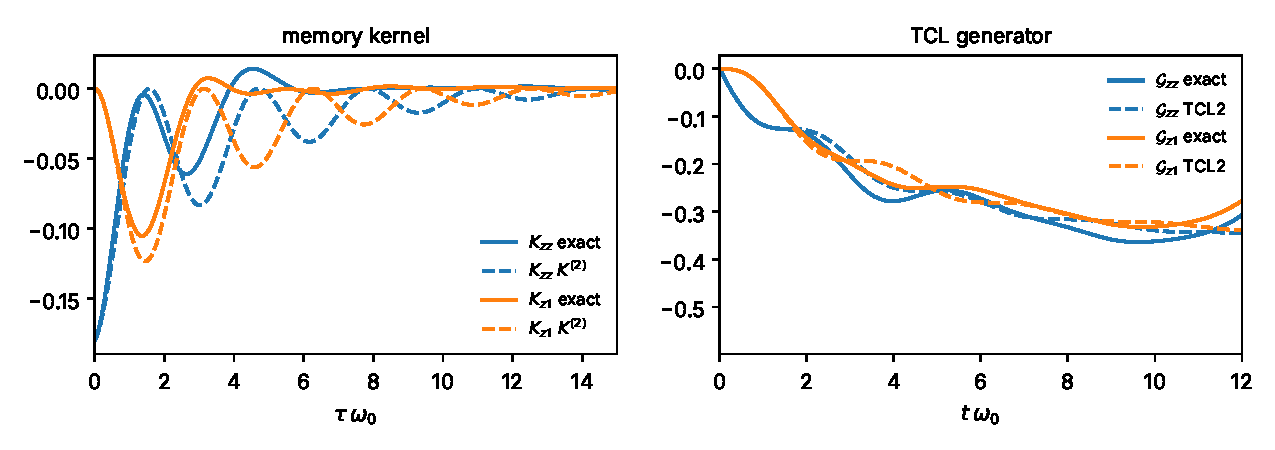
\includegraphics[width=\textwidth]{figures/fig_kernels.pdf}
\caption{Left: the exact NZ memory kernel of the Lorentzian model at $g=0.3$,
$\theta=\pi/4$ (elements $K_{zz}$ and $K_{z\Id}$ in the Bloch basis), compared with the Born
kernel $K^{(2)}$. Right: the exact TCL generator $\Gc(t)=\dot\Pi\Pi^{-1}-\Lc_S$ compared
with the TCL2 generator $\Gc^{(2)}(t)$ (\cref{sec:lec6}). Both agree at short times by
construction; the exact generator develops large excursions near $t\omega_0\approx12$ where
$\Pi(t)$ becomes nearly singular.}
\label{fig:kernels}
\end{figure}

\subsection{Correlated initial states and the inhomogeneity}

If $\rho(0)$ is not factorized, $I(t)$ in \cref{eq:NZ} is nonzero. It decays on the bath
correlation time if the initial correlations are short-ranged, and it can be absorbed
into a modified kernel in some cases. In the Keldysh language the same information lives
on the imaginary-time (Matsubara) branch attached to the contour at
$t=0$~\cite[Ch.~4]{StefanucciVanLeeuwen}. One should not expect $\Pi(t)$ to be a
completely positive map of $\rhoS(0)$ in that case~\cite{Pechukas1994}.

\subsection{Exercises}

\begin{exercise}\label{ex:5-1}
Carry out the derivation of \cref{eq:NZ} with a general projector $\Pc$ (not necessarily
of the form \eqref{eq:P}) and identify which steps use $\Pc\Lc_I\Pc=0$ and $[\Pc,\Lc_0]=0$. What
changes if $\avg{B}\ne0$? (Hint: absorb $S\avg{B}$ into $H_S$.)
\end{exercise}

\begin{exercise}\label{ex:5-2}
Derive the Bloch equations \eqref{eq:bloch-eqs}--\eqref{eq:lamb} from \cref{eq:K2-bloch}.
Show that the real part of the response, $\chi'$, cancels from $\delta\omega$ and explain why
with a parity argument. Then obtain the same rates from the operator form
$\Gc X=-i[H_S+H_{\rm LS},X]+\sum_\omega\gamma(\omega)\big(A(\omega)XA(\omega)^\dagger-\tfrac12\{A(\omega)^\dagger A(\omega),X\}\big)$ with
$A(\pm\omega_0)=\sin\theta\,\sigma_\mp$, $A(0)=\cos\theta\,\sz$, $\gamma(\omega)=C(\omega)$~\cite[Sec.~3.3.1]{BreuerPetruccione}.
\end{exercise}

\begin{exercise}\label{ex:5-3}
Show that the secular generator of \cref{ex:5-2} is of GKSL form with
$L_1=\sigma_-$, $L_2=\sigma_+$, $L_3=\sz$ and nonnegative rates. Then take the nonsecular
Redfield generator for $\theta=\pi/2$ and find an initial state and a time at which
$\Tr\rhoS^2>1$ for a Lorentzian bath with $\gamma\gtrsim\omega_0$.
\end{exercise}

\begin{exercise}\label{ex:5-4}
Prove $K(0)=K^{(2)}(0)$ directly from \cref{eq:NZ}. Then show that in Laplace space
$\hat K(z)=z-\Lc_S-\hat\Pi(z)^{-1}$, so that the exact kernel can be \emph{extracted} from the
exact map (this is the route of Shi and Geva~\cite{ShiGeva2003} and of Cohen and
Rabani~\cite{CohenRabani2011}). Use it to show that for pure dephasing ($\theta=0$) the
coherence kernel $\hat K_{01}(z)$ is an infinite series in $g^2$ even though the exact
solution \eqref{eq:dephasing-exact} is ``second order'' in a different sense.
\end{exercise}

\clearpage
